\chapter{Korrektheit}


%Aussageformeln vergleichen bei semantischer gleichheit von Code und Diffs
%Am Anfang allgemein zum vergleichen erzählen mit Tabelle für beide Datenschtrukturen und Varianten. Danach Zwei unter Kapietel für jede DatenStruktur wo man genauer auf symantische Gleichheit eingeht, andere kann man erwähnen aber sie sind bei beiden sehr ähnlich
%oder nach dem anfang unterkapietel für jede Art des Vergleichs machen , wie Groß muss so ein Unterkapietel sein? Bei semantischer gleichheit vileicht Unterunterkapiel für datenstrukturen
\section{Korrektheitskritierum}

In diesem Kapitel stellen wir die Metrik vor, an der wir die Korrektheit unserer Lösung betrachten wollen. Dieser Kapitel beschäftigt sich nur mit Arten der Korrektheit und wie diese als Konzept für textbasierte Diffs und mit C-Präprozessor-Annotierten Code funktionieren soll. Die drei Arten der Korrektheit für textbasierte Diffs und mit C-Präprozessor-Annotierten Code, sind syntaktische Korrektheit, syntaktische Korrektheit ohne Whitespace und semantische Korrektheit, werden in diesem Kapitel erläutert.\\


Nachdem wir eine algorithmische Lösung für das Problem ausgearbeitet haben, müssen wir entscheiden, ob unsere Lösung korrekt ist. Um die Kriterien, an den die Korrektheit festgelegt wird, wird es in folgenden gehen. Wir stellen Ihnen unsere Metrik für die Korrektheit des Unparsens. Wir haben uns für drei mögliche Arten der Korrektheit entschieden, an denen wir die Korrektheit entscheiden. Diese Arten sind syntaktische Gleichheit, syntaktische Gleichheit ohne Whitespace und semantische Gleichheit. Wenn die ausgangs Eingabe und das Ergebnis der ausgangs Eingabe nach Parsen und Unparsen eine dieser Gleichheiten erfühlen gilt das Unparsen für diesen Fall als Korrekt. In der Tabelle 4.1 ist kurz zusammengefasst wie jeweils die Art der Korrektheit bezogen auf C-Präprozessor-Annotierter Code oder textbasierte Diffs zu verstehen sind.

\begin{table}[H]
	
	\begin{center}
		\begin{tabular}{ c||c|c|c| } 
			& \parbox[][2.5cm][]{4cm}{Variation-Tree\\ \hspace*{1cm} $\downarrow$ \\ C-Präprozessor-Annotierter Code} & \parbox[][][]{4cm}{Variation-Diff\\ \hspace*{1cm} $\downarrow$ \\ textbasierter Diff} \\ 
			\hline
			Syntaktische Gleichheit & \parbox[][3.5cm][]{5cm}{Sei $C$ die Menge aller mit C-Präprozessor-Annotierter Codes und $VT$ die Menge aller Variation-Trees.\\
				$parse_t$ : $C$ $\rightarrow$ $VT$\\
				$unparse_t$ : $VT$ $\rightarrow$ $C$\\
				$unparse_t$ $\circ$ $parse_t$ = $id$} & \parbox[][3.5cm][]{5cm}{Sei $D$ die Menge aller textbasierter  Diffs und $VD$ die Menge aller Variation-Diffs.\\
				$parse_d$ : $D$ $\rightarrow$ $VD$\\
				$unparse_d$ : $VD$ $\rightarrow$ $D$\\
				$unparse_d$ $\circ$ $parse_d$ = $id$} \\ 
			\hline
			\parbox[][1cm][]{4cm}{Syntaktische Gleichheit ohne Whitespace} & \parbox[][5.5cm][]{5.3cm}{Sei $C$ die Menge aller mit C-Präprozessor-Annotierter Codes, $VT$ die Menge aller Variation-Trees und $T$ Menge aller Texte.\\
				$parse_t$ : $C$ $\rightarrow$ $VT$\\
				$unparse_t$ : $VT$ $\rightarrow$ $C$\\
				$deleteWhitespace$ : $C$ $\rightarrow$ $T$\\
				$deleteWhitespace$ $\circ$ $unparse_t$ $\circ$ $parse_t$ = $deleteWhitespace$ $\circ$ $id$} & \parbox[][5.5cm][]{5.3cm}{Sei $D$ die Menge aller textbasierter Diffs, $VD$ die Menge aller Variation-Diffs und $T$ Menge aller Texte.\\
				$parse_d$ : $D$ $\rightarrow$ $VD$\\
				$unparse_d$ : $VD$ $\rightarrow$ $D$\\
				$deleteWhitespace$ : $D$ $\rightarrow$ $T$ \\ 
				$deleteWhitespace$ $\circ$ $unparse_d$ $\circ$ $parse_d$ = $deleteWhitespace$ $\circ$ $id$ } \\
			\hline
			Semantische Gleichheit &  \parbox[][3cm][]{4cm}{Out of Scope\\
				unentscheidbar für C,\\
				exponentielles Wachstum für C-Präprozessor}  &  \parbox[][10.5cm][]{5cm}{Sei $C$ die Menge aller mit C-Präprozessor-Annotierter Codes, $D$ die Menge aller textbasierter Diffs, $VT$ die Menge aller Variation-Trees,  $VD$ die Menge aller Variation-Diffs, $Z$=$\{\textcolor{green}{a},\textcolor{orange}{b}\}$ die Menge mit den Zeiten Davor und Danach und $T$ Menge aller Texte.\\
				$parse_d$ : $D$ $\rightarrow$ $VD$\\
				$unparse_d$ : $VD$ $\rightarrow$ $D$\\
				$deleteWhitespace$ : $C$ $\rightarrow$ $T$\\
				$textProject$ : ($D$,$Z$) $\rightarrow$ $C$\\
				Für $\forall t \in \{\textcolor{green}{a},\textcolor{orange}{b}\}$\\
				$textProject$($unparse_d$ $\circ$ $parse_d$,$t$) = $textProject$($id$,$t$) $\lor$ $deleteWhitespace$ $\circ$ $textProject$($unparse_d$ $\circ$ $parse_d$,$t$) =  $deleteWhitespace$ $\circ$ $textProject$($id$,$t$)
			} \\
			\hline
		\end{tabular}
	\end{center}
	\caption{Korrektheitskritien}
\end{table}


In diesem Abschnitt sprechen wir über die syntaktische Korrektheit, die zweite Zeile aus der Tabelle 4.1. Syntaktische Korrektheit bedeutet, dass der zu vergleichende Text in jedem Zeichen identisch ist. Der Vergleich auf syntaktische Korrektheit sieht für C-Präprozessorbasierten Code und textbasierte Diffs darauf gleich aus, was in der Abbildung 4.1 zu sehen ist. Hierfür muss der Ausgangs C-Präprozessor-Annotierter Code bzw. der textbasierter Diff mit dem Ergebnis nach dem Parsen und Unparsen in jedem Zeichen übereinstimmen. Wie in der Abbildung 4.1 wird ein C-Präprozessor-Annotierter Code bzw. der textbasierte Diff genommen, dann darauf Parser und Unparser angewendet. Das Ergebnis und der C-Präprozessor-Annotierter Code bzw. der textbasierte Diff wird dann jeweils in ein String umgewandelt und diese dann auf Gleichheit geprüft. So wird die syntaktische Gleichheit von den C-Präprozessor-Annotierten Code bzw. den textbasierten Diff und dem Ergebnis von Parser und Unparser überprüft.

\begin{figure}[H]
\centering
\begin{tikzpicture}
	\node[align=left,rectangle split,draw,rectangle split parts=2] (A) at (0,0) {\parbox{2cm}{\begin{singlespace}
				\#ifdef A \\ \hspace*{2mm} foo() \\ \#endif
	\end{singlespace}} \nodepart{two} \parbox{2cm}{\begin{singlespace}
	\#ifdef A \\ \hspace*{2mm} +boo() \\ \hspace*{2mm} -foo() \\ \#endif
\end{singlespace}}};
		\node[rectangle split,draw,rectangle split parts=2] (B) at (0,-5) {S1 ='\#ifdef A$\backslash$n foo()$\backslash$n\#endif' \nodepart{two}S3 ='\#ifdef A$\backslash$n +boo()$\backslash$n -foo()$\backslash$n\#endif'};
	\draw[-{>[scale=2.5,
		length=6,
		width=3]},line width=0.7pt] (A) -- (B)  node[midway,sloped,above] {$toString$} ;
	
	
		\node[align=left,rectangle split,draw,rectangle split parts=2] (C) at (9,0) {\parbox{2cm}{\begin{singlespace}
				\#ifdef A \\ \hspace*{2mm} foo() \\ \#endif
		\end{singlespace}} \nodepart{two} \parbox{2cm}{\begin{singlespace}
				\#ifdef A \\ \hspace*{2mm} +boo() \\ \hspace*{2mm} -foo() \\ \#endif
	\end{singlespace}}};
	\node[rectangle split,draw,rectangle split parts=2] (D) at (9,-5) {S2 ='\#ifdef A$\backslash$n foo()$\backslash$n\#endif'\nodepart{two}S4 ='\#ifdef A$\backslash$n +boo()$\backslash$n -foo()$\backslash$n\#endif'};
	\draw[-{>[scale=2.5,
		length=6,
		width=3]},line width=0.7pt] (C) -- (D)  node[midway,sloped,above] {$toString$} ;
	
	\node[rectangle split,draw,rectangle split parts=2] (E) at (4.5,-8){equals(S1,S2) == True \nodepart{two} equals(S3,S4) == True};
	\draw[-{>[scale=2.5,
		length=6,
		width=3]},line width=0.7pt] (B) -- (E);
	\draw[-{>[scale=2.5,
		length=6,
		width=3]},line width=0.7pt] (D) -- (E);
	
	\draw[-{>[scale=2.5,
		length=6,
		width=3]},line width=0.7pt] (A) -- (C)  node[midway,sloped,above] {$Parse$ und $Unparse$ Schritt} ;
	
\end{tikzpicture}
\caption{Beispiel für Syntaktische Gleichheit }
\end{figure}

Der syntaktischen Korrektheit ohne Whitespace aus der dritten Zeile der Tabelle 4.1 widmen wir uns in diesem Abschnitt. Analog zu syntaktischer Gleichheit ist syntaktische Gleichheit ohne Whitespace für den C-Präprozessor-Annotierten Code und textbasierte Diffs gleich zu verstehen, wie in Abbildung 4.2 zu sehen ist. Bei dieser Art von Korrektheit muss auch wie in vorherigen Fall der ausgangs C-Präprozessor-Annotierter Code bzw. der textbasierter Diff mit dem Ergebnis nach dem Parsen und Unparsen Schritt in jedem Zeichen übereinstimmen, aber nur nachdem alle Zeichen, die zu Gruppe der Whitespace-Zeichen gehören, entfernt wurden. Die Abbildung 4.2 veranschaulicht das. Dort sind der ausgangs C-Präprozessor-Annotierter Code bzw. der textbasierte Diff gegeben. Links von den ist das Ergebnis von Parse und Unparse Schritt. Danach werden die alle in Strings umgewandelt. Als Nächstes werden alle Whitespace-Zeichen aus den Strings entfernt und anschließend die auf Äquivalenz geprüft. So wird der C-Präprozessor-Annotierter Code bzw. der textbasierte Diff und das Ergebnis von Parse und Unparse Schritt auf syntaktische Gleichheit ohne Whitespace überprüft.

\begin{figure}[H]
	\centering
	\begin{tikzpicture}
		\node[align=left,rectangle split,draw,rectangle split parts=2] (A) at (0,0) {\parbox{2cm}{\begin{singlespace}
					\#ifdef A \\ \hspace*{2mm} foo() \\ \#endif
			\end{singlespace}} \nodepart{two} \parbox{2cm}{\begin{singlespace}
					\#ifdef A \\ \hspace*{2mm} +boo() \\ \hspace*{2mm} -foo() \\ \\ \#endif
		\end{singlespace}}};
		\node[rectangle split,draw,rectangle split parts=2] (B) at (0,-5.5) {S1 ='\#ifdef A$\backslash$n foo()$\backslash$n\#endif' \nodepart{two}S3 ='\#ifdef A$\backslash$n +boo()$\backslash$n -foo()$\backslash$n$\backslash$n\#endif'};
		\draw[-{>[scale=2.5,
			length=6,
			width=3]},line width=0.7pt] (A) -- (B)  node[midway,sloped,above] {$toString$} ;
			
		\node[rectangle split,draw,rectangle split parts=2] (F) at (0,-8) {S1 ='\#ifdefAfoo()\#endif'\nodepart{two}S3 ='\#ifdefA+boo()-foo()\#endif'};	
			
			
			
			
		
		
		\node[align=left,rectangle split,draw,rectangle split parts=2] (C) at (9,0) {\parbox{2cm}{\begin{singlespace}
					\#ifdef A \\ \hspace*{2mm} foo() \\ \\ \#endif
			\end{singlespace}} \nodepart{two} \parbox{2cm}{\begin{singlespace}
					\#ifdef A \\ \hspace*{2mm} +boo() \\ \hspace*{2mm} -foo() \\ \#endif
		\end{singlespace}}};
		\node[rectangle split,draw,rectangle split parts=2] (D) at (9,-5.5) {S2 ='\#ifdef A$\backslash$n foo()$\backslash$n$\backslash$n\#endif'\nodepart{two}S4 ='\#ifdef A$\backslash$n +boo()$\backslash$n -foo()$\backslash$n\#endif'};
		\draw[-{>[scale=2.5,
			length=6,
			width=3]},line width=0.7pt] (C) -- (D)  node[midway,sloped,above] {$toString$} ;
			
		\node[rectangle split,draw,rectangle split parts=2] (G) at (9,-8) {S2 ='\#ifdefAfoo()\#endif'\nodepart{two}S4 ='\#ifdefA+boo()-foo()\#endif'};
			
			
		
		
		\node[rectangle split,draw,rectangle split parts=2] (E) at (4.5,-10){equals(S1,S2) == True \nodepart{two} equals(S3,S4) == True};
		\draw[-{>[scale=2.5,
			length=6,
			width=3]},line width=0.7pt] (B) -- (F);
		\draw[-{>[scale=2.5,
			length=6,
			width=3]},line width=0.7pt] (D) -- (G);
			
		\draw[-{>[scale=2.5,
			length=6,
			width=3]},line width=0.7pt] (G) -- (E);
			
		\draw[-{>[scale=2.5,
			length=6,
			width=3]},line width=0.7pt] (F) -- (E);
		
		\draw[-{>[scale=2.5,
			length=6,
			width=3]},line width=0.7pt] (A) -- (C)  node[midway,sloped,above] {$Parse$ und $Unparse$ Schritt} ;
		
	\end{tikzpicture}
	\caption{Beispiel für Syntaktische Gleichheit ohne Whitespace }
\end{figure}

Die semantische Gleichheit von mit C-Präprozessor-Annotierten Code werden wir nicht betrachten, da dafür wir entscheiden müssen ab zwei Programmen äquivalent sind. Das geht über den Rand unserer Möglichkeiten, da diese Fragestellung unentscheidbar ist und als das Äquivalenzproblem bekannt~\cite{Fischer1972}. Mit den C-Präprozessor-Annotationen geht es auch über den Rand unserer Möglichkeiten, da C-Präprozessor-Annotationen hier für Erzeugung der Variabilität verwendet werden. Dabei hat so eine Softwareproduktlinie n Features und im Worst-Case muss $2^n$ Varianten der Software betrachtet werden\cite{ABKS13}, welches eine exponentielle Laufzeit bedeutet und über den Rand unserer Möglichkeiten geht.\\




Um die semantische Gleichheit für textbasierte Diffs geht es in diesem Abschnitt. Wie die semantische Gleichheit für textbasierte Diffs zu verstehen ist, ist nicht eindeutig festgelegt. Unsere Interpretation der semantischen Gleichheit für textbasierte Diffs ist an der Gleichheit für Variation-Diffs~\cite{BSG+:SPLC23} orientiert. Wir verstehen die semantische Gleichheit wie folgt, zwei textbasierte Diffs sind semantisch gleich, wenn ihre Projektionen auf den Zustand davor bzw. danach syntaktisch gleich oder syntaktisch gleich ohne Whitespace sind. In der Abbildung 4.3 ist dies dargestellt. Dabei ist die Projektion für textbasierte Diffs wie folgt zu verstehen: Ein textbasierter Diff hat Zeilen von drei Typen unverändert gebliebene Zeilen, gelöschte Zeilen und eingefügte Zeilen. Bei der Projektion werden einige dieser Typen der Zeilen entfernt einige beibehalten und so entsteht eine Projektion von textbasierten Diff auf ein mit C-Präprozessor-Annotierten Code. Dabei wird für die Projektion auf den Zustand davor, die unveränderten und gelöschten Zeilen beibehalten und die eingefügten entfernt und für die Projektion auf den Zustand danach, die unveränderten und eingefügten Zeilen beibehalten und die gelöschten Zeilen entfernt. Dies verläuft analog zu der Projektion von Variation-Diff zu Variation-Tree.

\begin{figure}[H]
	\centering
	\begin{tikzpicture}
		\node[draw,align=left] (U) at (-1,-11) {\parbox{2cm}{\begin{singlespace}
					\#ifdef A \\ \hspace*{2mm} +boo() \\ \hspace*{2mm} -foo() \\ \#endif
		\end{singlespace}}};
		\node[draw,align=left] (V) at (9,-11) {\parbox{2cm}{\begin{singlespace}
					\#ifdef A \\ \hspace*{2mm} -foo() \\ \hspace*{2mm} +boo() \\ \#endif
		\end{singlespace}}};
		\node[draw,align=left] (Z) at (4,-8.5) {\parbox{2cm}{\begin{singlespace}
					\#ifdef A \\ \hspace*{2mm} foo() \\ \#endif
		\end{singlespace}}};
		\node[draw,align=left] (X) at (4,-13.5) {\parbox{2cm}{\begin{singlespace}
					\#ifdef A \\ \hspace*{2mm} boo() \\ \#endif
		\end{singlespace}}};
	
		\node[draw,align=center] (A) at (4,-6) {Syntaktische Gleichheit == True\\ $\lor$ \\ Syntaktische Gleichheit ohne Whitespace == True};
	
		\node[draw,align=center] (B) at (4,-16) {Syntaktische Gleichheit == True\\ $\lor$ \\ Syntaktische Gleichheit ohne Whitespace == True};
	
	
		\draw[-{>[scale=2.5,
			length=6,
			width=3]},line width=0.7pt] (U) -- (Z) node[midway,sloped,above] {$projectBefore$};
		\draw[-{>[scale=2.5,
			length=6,
			width=3]},line width=0.7pt] (U) -- (X) node[midway,sloped,above] {$projectAafter$};
		\draw[-{>[scale=2.5,
			length=6,
			width=3]},line width=0.7pt] (V) -- (Z) node[midway,sloped,above] {$projectBefore$};
		\draw[-{>[scale=2.5,
			length=6,
			width=3]},line width=0.7pt] (V) -- (X) node[midway,sloped,above] {$projectAfter$};
			
		\draw[-{>[scale=2.5,
			length=6,
			width=3]},line width=0.7pt] (Z) -- (A) ;
			
		\draw[-{>[scale=2.5,
			length=6,
			width=3]},line width=0.7pt] (X) -- (B) ;
			
		\draw[-{>[scale=2.5,
			length=6,
			width=3]},line width=0.7pt] (U) -- (V) node[midway,sloped,above] {$Parse$ und $Unparse$ Schritt};
			
	\end{tikzpicture}
	\caption{Beispiel für Semantische Gleichheit }
\end{figure}


Im Weiteren wollen wir besprächen wie die Korrektheitskriterien zusammenhängen. Bevor wir aber dazu kommen, Hilfsaussagen erläutert. Bei Syntaktischer Gleichheit und Syntaktischen Gleichheit ohne Whitespace für mit C-Präprozessor-Annotierten Code und textbasierten Diffs werden im Grunde genommen nur Texte verglichen. Aus diesem Grund wird für die Beschreibung der Zusammenhänge zwischen Syntaktischer Gleichheit und Syntaktischen Gleichheit ohne Whitespace nur auf Text eingegangen und nicht zwischen mit C-Präprozessor-Annotierten Code und textbasierten Diffs unterschieden.

Der Zusammenhang zwischen Syntaktischer Gleichheit und Syntaktischen Gleichheit ohne Whitespace ist folgender. Die Syntaktische Gleichheit impliziert Syntaktischen Gleichheit ohne Whitespace. Diese Aussage stimmt, da Syntaktische Gleichheit bedeutet das die zwei zu vergleichende Texte in jedem Zeichen und der Position dieser Zeichen identisch sind. Wenn aus den syntaktisch Gleichen Texten alle Whitespace Zeichen entfernt werden, sind diese Texte trotzdem syntaktisch Gleich. Der Grund dafür ist das bei zwei syntaktisch Gleichen Texten alle Whitespace Zeichen an den selben Stellen sind und das nach deren Entfernung alle anderen Zeichen, welche in beiden Texten gleich sind, auch in beiden Texten identisch verschoben werden und damit auch Syntaktischen Gleichheit ohne Whitespace besitzen. Damit gilt die Aussage.

\section{Auswertung}

Im folgenden Abschnitt wollen wir eine Auswertung unserer Implementierung anhand der vorher eingeführten Korrektheitskriterien durchführen. Bei dieser Auswertung wollen wir herausfinden welche Korrektheitskriterien wie oft eingehalten werden und wird mindestens eine der Kriterien eingehalten oder gibt es Fälle, welcher unser Unparser nicht nach unserer Definition korrekt Unparsen kann. Dazu hat DiffDetective für das Parsen zwei unabhängige Optionen, dass sind Collabse-Multiple-Code-Lines und Ignore-Empty-Lines. Bei Collabse-Multiple-Code-Lines werden mehrere hintereinander Laufende Zeilen von Code und nicht von C-Präprozessor-Annotationen in einem Knoten zusammengefasst. Bei Ignore-Empty-Lines werden die leeren Zeilen nicht von Parser in das Ergebniss aufgenommen und gehen verloren. Es gibt vier Möglichkeiten, wie die Optionen für den Parser gesetzt werden können. Für alle diese Möglichkeiten wollen wir betrachten, wie die Korrektheitskriterien eingehalten werden.\\

Zuerst im Abschnitt 5.2.1 wird der Aufbau des Experiments vorgestellt. Danach sind die Ergebnisse der Auswertung in Abschnitt 5.2.2 zu sehen. Zum Schluss im Abschnitt 5.2.3 werden die Ergebnisse der Auswertung interpretiert und diskutiert.

%Vorschungs Frage : ist Implementierung Korrekt, welche Korrektheitskriterien werden erfüllt

\subsection{Aufbau des Experiments}
Bei der Auswertung wird DiffDetective uns seine Möglichkeiten zur Analyse von Software-Produkt-Linien verwendet. Der Aufbau unserer Auswertung ist in der Abbildung 5.4 skizziert und ist folgend aufgebaut. Es wird automatisch die Patches aus dem Git Repositorie extrahiert. Wir arbeiten nur mit Patches, welche geparst werden können, die Patches bei denen es nicht gilt ignorieren wir, da diese für unsere Fragestellung unbedeutend sind. Wir wollen die Korrektheit des Unparser prüfen, also die Fällen wo wir keinen Variation-Tree oder Variation-Diff bekommen können, müssen wir nicht betrachten. Wenn wir dann so ein Patch/textbasierten Diff haben, wird dieser auf den Davor-Zustand und Danach-Zustand projiziert. Damit erhalten wir dann zwei C-Präprozessor-Annotierte Codes. Dadurch wird bei der Auswertung doppelt so viele C-Präprozessor-Annotierte Codes untersucht als textbasierte Diffs. Als nächstes wird sowohl für der textbasierter Diff als auch C-Präprozessor-Annotierte Code geparst. Dabei werden für ein textbasierten Diff und ein C-Präprozessor-Annotierten Code vier Variation-Diffs bzw. Variation-Trees erstellt. Aus einem Patch bekommen wir aber zwei C-Präprozessor-Annotierte Codes und diese werden zusammen mit den textbasierten Diff untersucht, dadurch bekommen wir acht Variation-Trees. Diese vier Variation-Diffs und acht Variation-Trees werden unter Verwendung verschiedener Optionen erstellt. Es gibt zwei unabhängige Optionen für den Parser, diese erzeugen dann die vier möglichen Kombinationen. Danach werden diese vier Variation-Diffs und acht Variation-Trees ungepasrt und wir erhalten danach vier textbasierte Diffs und auch C-Präprozessor-Annotierte Codes. Diese textbasierten Diffs und C-Präprozessor-Annotierte Codes werden dann auf die Gleichheit mit den ausgangs textbasierten Diff und C-Präprozessor-Annotierte Codes, welche für das Parsen verwendet wurden, anhand der von uns definierten Korrektheitskriterien geprüft. Die Ergebnisse nach der Untersuchung aller für uns geltender Patches werden zusammen getragen und wir können dann diese betrachten.\\

Als Datenquelle werden von uns Git-History folgende vier Software-Produkt-Linie Projekte benutzt. Die verwendeten Open-Source Projekte sind Vim, sylpheed, gcc und berkeley-db-libdb. Vim ist ein konfigurierbarer Texteditor, welcher auch in den meisten UNIX-Systemen und in Apple OS X enthalten ist. sylpheed ist ein leichtgewichtiger E-Mail-Client, welcher auf vielen Systemen wie Windows, Linux, BSD, Mac OS X und anderen Unix-ähnlichen Systemen läuft. gcc steht für GNU Compiler Collection, welcher eine Sammlung von Compilern ist für die Programmiersprachen C, C++, Objective-C, D, Fortran, Ada und Go. berkeley-db-libdb ist eine eingebetteten Key-Value-Datenbankbibliothek. Aus diesen Projekten haben wir nur Dateien mit C-Code untersucht. Diese Dateien sind an den Endungen .c und .cpp zu erkennen. 

%-Nutzen DiffDetective
\begin{figure}[h]
	\centering
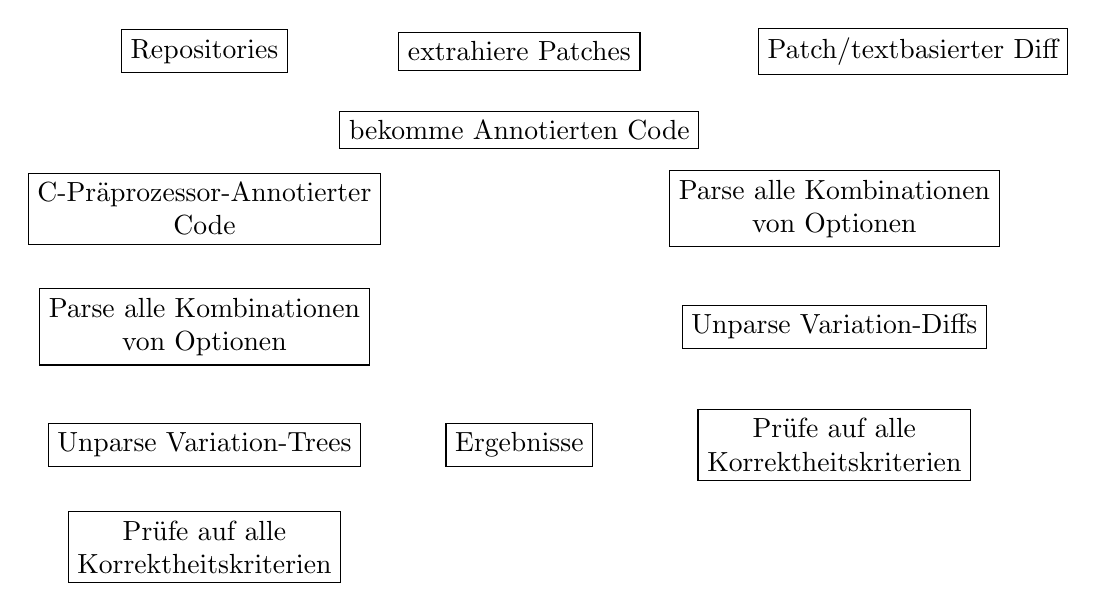
\begin{tikzpicture}
	\node[draw,align=center] (A) at (0,0) {Repositories};
	\node[draw,align=center] (B) at (4,0) {extrahiere Patches};
	\node[draw,align=center] (C) at (9,0) {Patch/textbasierter Diff};
	\node[draw,align=center] (B) at (4,-1) {bekomme Annotierten Code};
	\node[draw,align=center] (E) at (0,-2) {C-Präprozessor-Annotierter\\ Code};
	\node[draw,align=center] (F) at (8,-2) {Parse alle Kombinationen \\von Optionen};
	\node[draw,align=center] (G) at (8,-3.5) {Unparse  Variation-Diffs};
	\node[draw,align=center] (H) at (8,-5) {Prüfe auf alle\\Korrektheitskriterien};
	\node[draw,align=center] (I) at (0,-3.5) {Parse alle Kombinationen \\von Optionen};
	\node[draw,align=center] (J) at (0,-5) {Unparse  Variation-Trees};
	\node[draw,align=center] (K) at (0,-6.3) {Prüfe auf alle\\Korrektheitskriterien};
	\node[draw,align=center] (L) at (4,-5) {Ergebnisse};
\end{tikzpicture}
\caption{Aufbau der Auswertung}
\end{figure}

\subsection{Ergebnisse}

\subsection{Diskussion}
%interpretation der Ergebnisse
%Beantworten der Forschungsfrage

\section{Zusammenfassung}










